\documentclass{article}
\usepackage{tikz}
\usepackage{CJKutf8}
\usepackage{amsmath}
\usepackage{amsthm}
\begin{document}
\title{第七章作业题}
\begin{CJK}{UTF8}{gbsn}
  \newtheorem*{Exercise}{习题}
  \date{}
  \maketitle

  \begin{Exercise}
  分别画出具有$4$个,$5$个,$6$个,$7$个顶点的所有树(同构的只算一个)。
\end{Exercise}

  \begin{proof}[解]
  具有$4$个顶点的所有互不同构的树:
  \vspace{0.5cm}
  
    
  \begin{minipage}{0.5\linewidth}
    \centering
    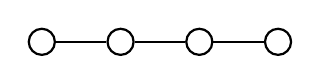
\begin{tikzpicture}[auto,
    specification/.style ={circle, draw, thick}]
   \node[specification] (A) at (0,0)  {};
   \node[specification] (B)  at (1,0)  {};
   \node[specification] (C)  at (2,0)  {};
   \node[specification] (D) at (3,0)  {};
   \draw[thick] (A) to  (B);
   \draw[thick] (B) to  (C);
   \draw[thick] (C) to  (D);
 \end{tikzpicture}
\end{minipage}
\begin{minipage}{0.5\linewidth}
    \centering
    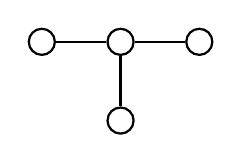
\begin{tikzpicture}[auto,
    specification/.style ={circle, draw, thick}]
   \node[specification] (A) at (0,0)  {};
   \node[specification] (B)  at (1,0)  {};
   \node[specification] (C)  at (2,0)  {};
   \node[specification] (D) at (1,-1)  {};
   \draw[thick] (A) to  (B);
   \draw[thick] (B) to  (C);
   \draw[thick] (B) to  (D);
 \end{tikzpicture}
\end{minipage}

具有$5$个顶点的所有互不同构的树:
  \vspace{0.5cm}

  \begin{minipage}{0.5\linewidth}
    \centering
    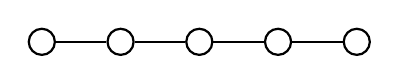
\begin{tikzpicture}[auto,
    specification/.style ={circle, draw, thick}]
   \node[specification] (A) at (0,0)  {};
   \node[specification] (B)  at (1,0)  {};
   \node[specification] (C)  at (2,0)  {};
   \node[specification] (D) at (3,0)  {};
   \node[specification] (E) at (4,0)  {};
   
   \draw[thick] (A) to  (B);
   \draw[thick] (B) to  (C);
   \draw[thick] (C) to  (D);
   \draw[thick] (D) to  (E);
 \end{tikzpicture}
\end{minipage}
  \begin{minipage}{0.5\linewidth}
    \centering
    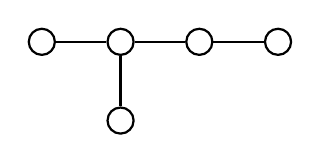
\begin{tikzpicture}[auto,
    specification/.style ={circle, draw, thick}]
   \node[specification] (A) at (0,0)  {};
   \node[specification] (B)  at (1,0)  {};
   \node[specification] (C)  at (2,0)  {};
   \node[specification] (D) at (3,0)  {};
   \node[specification] (E) at (1,-1)  {};
   
   \draw[thick] (A) to  (B);
   \draw[thick] (B) to  (C);
   \draw[thick] (C) to  (D);
   \draw[thick] (B) to (E);
 \end{tikzpicture}
\end{minipage}

  \begin{minipage}{0.5\linewidth}
    \centering
    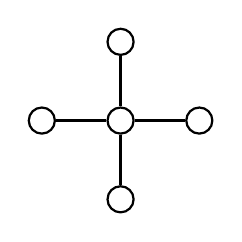
\begin{tikzpicture}[auto,
    specification/.style ={circle, draw, thick}]
   \node[specification] (A) at (0,0)  {};
   \node[specification] (B)  at (1,0)  {};
   \node[specification] (C)  at (2,0)  {};
   \node[specification] (D) at (1,1)  {};
   \node[specification] (E) at (1,-1)  {};
   
   \draw[thick] (A) to  (B);
   \draw[thick] (B) to  (C);
   \draw[thick] (B) to  (D);
   \draw[thick] (B) to (E);
 \end{tikzpicture}
\end{minipage}



具有$6$个顶点的所有互不同构的树:
  \vspace{0.5cm}

  \begin{minipage}{0.5\linewidth}
    \centering
    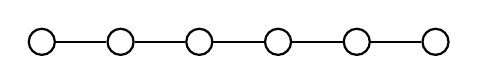
\begin{tikzpicture}[auto,
    specification/.style ={circle, draw, thick}]
   \node[specification] (A) at (0,0)  {};
   \node[specification] (B)  at (1,0)  {};
   \node[specification] (C)  at (2,0)  {};
   \node[specification] (D) at (3,0)  {};
   \node[specification] (E) at (4,0)  {};
   \node[specification] (F) at (5,0)  {};

   \draw[thick] (A) to  (B);
   \draw[thick] (B) to  (C);
   \draw[thick] (C) to  (D);
   \draw[thick] (D) to  (E);
   \draw[thick] (E) to  (F);   
 \end{tikzpicture}
\end{minipage}
  \begin{minipage}{0.5\linewidth}
    \centering
    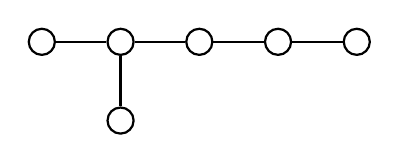
\begin{tikzpicture}[auto,
    specification/.style ={circle, draw, thick}]
   \node[specification] (A) at (0,0)  {};
   \node[specification] (B)  at (1,0)  {};
   \node[specification] (C)  at (2,0)  {};
   \node[specification] (D) at (3,0)  {};
   \node[specification] (E) at (4,0)  {};
   \node[specification] (F) at (1,-1)  {};

   \draw[thick] (A) to  (B);
   \draw[thick] (B) to  (C);
   \draw[thick] (C) to  (D);
   \draw[thick] (D) to  (E);
   \draw[thick] (B) to  (F);   
 \end{tikzpicture}
\end{minipage}

  \begin{minipage}{0.5\linewidth}
    \centering
    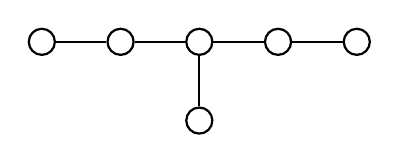
\begin{tikzpicture}[auto,
    specification/.style ={circle, draw, thick}]
   \node[specification] (A) at (0,0)  {};
   \node[specification] (B)  at (1,0)  {};
   \node[specification] (C)  at (2,0)  {};
   \node[specification] (D) at (3,0)  {};
   \node[specification] (E) at (4,0)  {};
   \node[specification] (F) at (2,-1)  {};

   \draw[thick] (A) to  (B);
   \draw[thick] (B) to  (C);
   \draw[thick] (C) to  (D);
   \draw[thick] (D) to  (E);
   \draw[thick] (C) to  (F);   
 \end{tikzpicture}
\end{minipage}
  \begin{minipage}{0.5\linewidth}
    \centering
    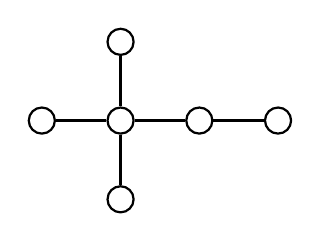
\begin{tikzpicture}[auto,
    specification/.style ={circle, draw, thick}]
   \node[specification] (A) at (0,0)  {};
   \node[specification] (B)  at (1,0)  {};
   \node[specification] (C)  at (2,0)  {};
   \node[specification] (D) at (3,0)  {};
   \node[specification] (E) at (1,1)  {};
   \node[specification] (F) at (1,-1)  {};

   \draw[thick] (A) to  (B);
   \draw[thick] (B) to  (C);
   \draw[thick] (C) to  (D);
   \draw[thick] (B) to  (E);
   \draw[thick] (B) to  (F);   
 \end{tikzpicture}
\end{minipage}

  \begin{minipage}{0.5\linewidth}
    \centering
    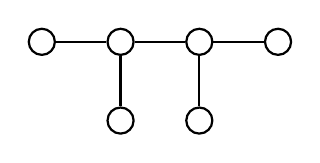
\begin{tikzpicture}[auto,
    specification/.style ={circle, draw, thick}]
   \node[specification] (A) at (0,0)  {};
   \node[specification] (B)  at (1,0)  {};
   \node[specification] (C)  at (2,0)  {};
   \node[specification] (D) at (3,0)  {};
   \node[specification] (E) at (2,-1)  {};
   \node[specification] (F) at (1,-1)  {};

   \draw[thick] (A) to  (B);
   \draw[thick] (B) to  (C);
   \draw[thick] (C) to  (D);
   \draw[thick] (C) to  (E);
   \draw[thick] (B) to  (F);   
 \end{tikzpicture}
\end{minipage}
  \begin{minipage}{0.5\linewidth}
    \centering
    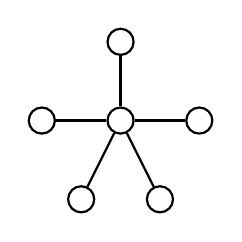
\begin{tikzpicture}[auto,
    specification/.style ={circle, draw, thick}]
   \node[specification] (A) at (0,0)  {};
   \node[specification] (B)  at (1,0)  {};
   \node[specification] (C)  at (2,0)  {};
   \node[specification] (D) at (1,1)  {};
   \node[specification] (E) at (0.5,-1)  {};
   \node[specification] (F) at (1.5,-1)  {};

   \draw[thick] (A) to  (B);
   \draw[thick] (B) to  (C);
   \draw[thick] (B) to  (D);
   \draw[thick] (B) to  (E);
   \draw[thick] (B) to  (F);   
 \end{tikzpicture}
\end{minipage}

  
具有$7$个顶点的所有互不同构的树:
  \vspace{0.5cm}

  \begin{minipage}{0.5\linewidth}
    \centering
    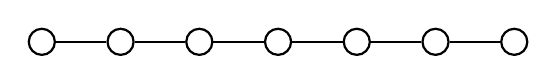
\begin{tikzpicture}[auto,
    specification/.style ={circle, draw, thick}]
   \node[specification] (A) at (0,0)  {};
   \node[specification] (B)  at (1,0)  {};
   \node[specification] (C)  at (2,0)  {};
   \node[specification] (D) at (3,0)  {};
   \node[specification] (E) at (4,0)  {};
   \node[specification] (F) at (5,0)  {};
   \node[specification] (G) at (6,0)  {};

   \draw[thick] (A) to  (B);
   \draw[thick] (B) to  (C);
   \draw[thick] (C) to  (D);
   \draw[thick] (D) to  (E);
   \draw[thick] (E) to  (F);
   \draw[thick] (F) to  (G);   
 \end{tikzpicture}
\end{minipage}
  \begin{minipage}{0.5\linewidth}
    \centering
    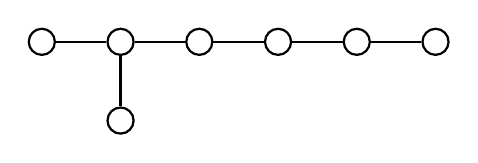
\begin{tikzpicture}[auto,
    specification/.style ={circle, draw, thick}]
   \node[specification] (A) at (0,0)  {};
   \node[specification] (B)  at (1,0)  {};
   \node[specification] (C)  at (2,0)  {};
   \node[specification] (D) at (3,0)  {};
   \node[specification] (E) at (4,0)  {};
   \node[specification] (F) at (5,0)  {};
   \node[specification] (G) at (1,-1)  {};

   \draw[thick] (A) to  (B);
   \draw[thick] (B) to  (C);
   \draw[thick] (C) to  (D);
   \draw[thick] (D) to  (E);
   \draw[thick] (E) to  (F);
   \draw[thick] (B) to  (G);   
 \end{tikzpicture}
\end{minipage}

\vspace{0.5cm}
  \begin{minipage}{0.5\linewidth}
    \centering
    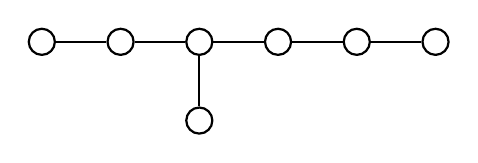
\begin{tikzpicture}[auto,
    specification/.style ={circle, draw, thick}]
   \node[specification] (A) at (0,0)  {};
   \node[specification] (B)  at (1,0)  {};
   \node[specification] (C)  at (2,0)  {};
   \node[specification] (D) at (3,0)  {};
   \node[specification] (E) at (4,0)  {};
   \node[specification] (F) at (5,0)  {};
   \node[specification] (G) at (2,-1)  {};

   \draw[thick] (A) to  (B);
   \draw[thick] (B) to  (C);
   \draw[thick] (C) to  (D);
   \draw[thick] (D) to  (E);
   \draw[thick] (E) to  (F);
   \draw[thick] (C) to  (G);   
 \end{tikzpicture}
\end{minipage}
\begin{minipage}{0.5\linewidth}
    \centering
    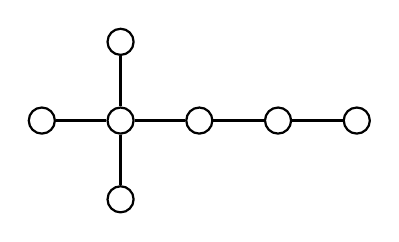
\begin{tikzpicture}[auto,
    specification/.style ={circle, draw, thick}]
   \node[specification] (A) at (0,0)  {};
   \node[specification] (B)  at (1,0)  {};
   \node[specification] (C)  at (2,0)  {};
   \node[specification] (D) at (3,0)  {};
   \node[specification] (E) at (4,0)  {};
   \node[specification] (F) at (1,-1)  {};
   \node[specification] (G) at (1,1)  {};

   \draw[thick] (A) to  (B);
   \draw[thick] (B) to  (C);
   \draw[thick] (C) to  (D);
   \draw[thick] (D) to  (E);
   \draw[thick] (B) to  (F);
   \draw[thick] (B) to  (G);   
 \end{tikzpicture}
\end{minipage}

\vspace{0.5cm}
\begin{minipage}{0.5\linewidth}
    \centering
    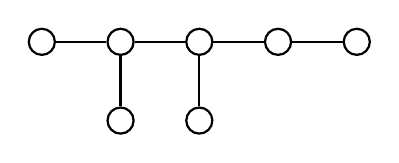
\begin{tikzpicture}[auto,
    specification/.style ={circle, draw, thick}]
   \node[specification] (A) at (0,0)  {};
   \node[specification] (B)  at (1,0)  {};
   \node[specification] (C)  at (2,0)  {};
   \node[specification] (D) at (3,0)  {};
   \node[specification] (E) at (4,0)  {};
   \node[specification] (F) at (1,-1)  {};
   \node[specification] (G) at (2,-1)  {};

   \draw[thick] (A) to  (B);
   \draw[thick] (B) to  (C);
   \draw[thick] (C) to  (D);
   \draw[thick] (D) to  (E);
   \draw[thick] (B) to  (F);
   \draw[thick] (C) to  (G);   
 \end{tikzpicture}
\end{minipage}
\begin{minipage}{0.5\linewidth}
    \centering
    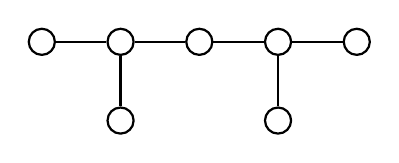
\begin{tikzpicture}[auto,
    specification/.style ={circle, draw, thick}]
   \node[specification] (A) at (0,0)  {};
   \node[specification] (B)  at (1,0)  {};
   \node[specification] (C)  at (2,0)  {};
   \node[specification] (D) at (3,0)  {};
   \node[specification] (E) at (4,0)  {};
   \node[specification] (F) at (1,-1)  {};
   \node[specification] (G) at (3,-1)  {};

   \draw[thick] (A) to  (B);
   \draw[thick] (B) to  (C);
   \draw[thick] (C) to  (D);
   \draw[thick] (D) to  (E);
   \draw[thick] (B) to  (F);
   \draw[thick] (D) to  (G);   
 \end{tikzpicture}
\end{minipage}

\vspace{0.5cm}
\begin{minipage}{0.5\linewidth}
    \centering
    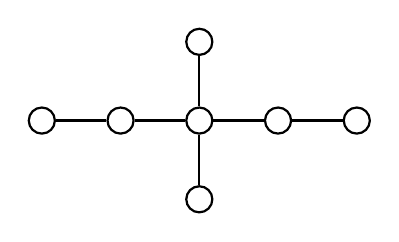
\begin{tikzpicture}[auto,
    specification/.style ={circle, draw, thick}]
   \node[specification] (A) at (0,0)  {};
   \node[specification] (B)  at (1,0)  {};
   \node[specification] (C)  at (2,0)  {};
   \node[specification] (D) at (3,0)  {};
   \node[specification] (E) at (4,0)  {};
   \node[specification] (F) at (2,-1)  {};
   \node[specification] (G) at (2,1)  {};

   \draw[thick] (A) to  (B);
   \draw[thick] (B) to  (C);
   \draw[thick] (C) to  (D);
   \draw[thick] (D) to  (E);
   \draw[thick] (C) to  (F);
   \draw[thick] (C) to  (G);   
 \end{tikzpicture}
\end{minipage}
\begin{minipage}{0.5\linewidth}
    \centering
    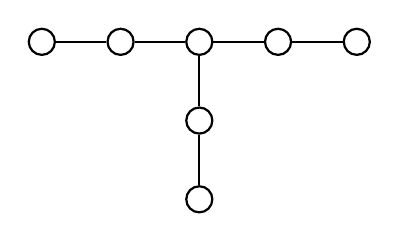
\begin{tikzpicture}[auto,
    specification/.style ={circle, draw, thick}]
   \node[specification] (A) at (0,0)  {};
   \node[specification] (B)  at (1,0)  {};
   \node[specification] (C)  at (2,0)  {};
   \node[specification] (D) at (3,0)  {};
   \node[specification] (E) at (4,0)  {};
   \node[specification] (F) at (2,-1)  {};
   \node[specification] (G) at (2,-2)  {};

   \draw[thick] (A) to  (B);
   \draw[thick] (B) to  (C);
   \draw[thick] (C) to  (D);
   \draw[thick] (D) to  (E);
   \draw[thick] (C) to  (F);
   \draw[thick] (F) to  (G);   
 \end{tikzpicture}
\end{minipage}

\vspace{0.5cm}
  \begin{minipage}{0.5\linewidth}
    \centering
    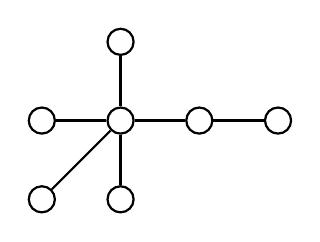
\begin{tikzpicture}[auto,
    specification/.style ={circle, draw, thick}]
   \node[specification] (A) at (0,0)  {};
   \node[specification] (B)  at (1,0)  {};
   \node[specification] (C)  at (2,0)  {};
   \node[specification] (D) at (3,0)  {};
   \node[specification] (E) at (1,1)  {};
   \node[specification] (F) at (0,-1)  {};
   \node[specification] (G) at (1,-1)  {};

   \draw[thick] (A) to  (B);
   \draw[thick] (B) to  (C);
   \draw[thick] (C) to  (D);
   \draw[thick] (B) to  (E);
   \draw[thick] (B) to  (F);
   \draw[thick] (B) to  (G);   
 \end{tikzpicture}
\end{minipage}
  \begin{minipage}{0.5\linewidth}
    \centering
    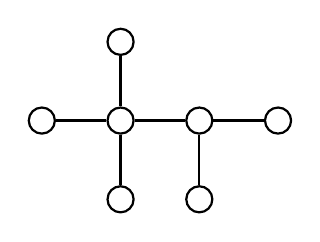
\begin{tikzpicture}[auto,
    specification/.style ={circle, draw, thick}]
   \node[specification] (A) at (0,0)  {};
   \node[specification] (B)  at (1,0)  {};
   \node[specification] (C)  at (2,0)  {};
   \node[specification] (D) at (3,0)  {};
   \node[specification] (E) at (1,1)  {};
   \node[specification] (F) at (2,-1)  {};
   \node[specification] (G) at (1,-1)  {};

   \draw[thick] (A) to  (B);
   \draw[thick] (B) to  (C);
   \draw[thick] (C) to  (D);
   \draw[thick] (B) to  (E);
   \draw[thick] (C) to  (F);
   \draw[thick] (B) to  (G);   
 \end{tikzpicture}
\end{minipage}

\vspace{0.5cm}
  \begin{minipage}{0.5\linewidth}
    \centering
    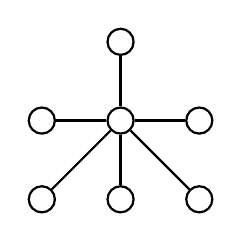
\begin{tikzpicture}[auto,
    specification/.style ={circle, draw, thick}]
   \node[specification] (A) at (0,0)  {};
   \node[specification] (B)  at (1,0)  {};
   \node[specification] (C)  at (2,0)  {};
   \node[specification] (D) at (1,1)  {};
   \node[specification] (E) at (0,-1)  {};
   \node[specification] (F) at (1,-1)  {};
   \node[specification] (G) at (2,-1)  {};

   \draw[thick] (A) to  (B);
   \draw[thick] (B) to  (C);
   \draw[thick] (B) to  (D);
   \draw[thick] (B) to  (E);
   \draw[thick] (B) to  (F);
   \draw[thick] (B) to  (G);   
 \end{tikzpicture}
\end{minipage}

  
\end{proof}

  \begin{Exercise}
  每个非平凡树是偶图。
\end{Exercise}

  \begin{proof}[证明]
  非平凡树中无圈,因此为偶图。
\end{proof}

  \begin{Exercise}
  设$G$为一棵树且$\Delta (G) \geq k$,证明$G$中至少有$k$个度为$1$的顶点。
\end{Exercise}

  \begin{proof}[证明]
  用反证法。假设$G$中有$x$个顶点,$x < k$。进一步,设$G$中有$p$个顶点,它们的度依次为$d_1$,$d_2$,$\ldots$,$d_p$。则
  \begin{equation*}
    \begin{split}
      \sum_{i=1}^pd_i &\geq k + x + 2(p-1-x)\\
      &= 2(p-1) + k - x\\
      &> 2(p-1)
    \end{split}
  \end{equation*}
  矛盾。
\end{proof}

  \begin{Exercise}令$G$是一个有$p$个顶点,$k$个支的森林,证明$G$有$p-k$条边。
\end{Exercise}

  \begin{proof}[证明]设$G$的$k$个支的顶点数依次为$p_1$,$p_2$,$\ldots$,$p_k$,边数依次为$q_1$,$q_2$,$\ldots$,$q_k$,则$q_1+q_2+\ldots + q_k=(p_1 - 1)+(p_2 - 1) +\ldots + (p_k - 1)$,即$q=p-k$。
\end{proof}

  \begin{Exercise}
  设树$T$中有$2n$个度为$1$的顶点,$3n$个度为$2$的顶点,$n$个度为$3$的顶点,那么这棵树有多少个顶点,多少条边呢?
\end{Exercise}

  \begin{proof}[证明]
  在树$T$中,边数=顶点数-1,从而$(2n\times 1 + 3n \times 2 + n \times 3)/2 = 2n + 3n + n - 1$,解得$n=2$,顶点数=12,边数=11。
\end{proof}

  \begin{Exercise}
  一棵非平凡树$T$有$n_2$个度为$2$的顶点,$n_3$个度为$3$的顶点,$\ldots$,$n_k$个度为$k$的顶点,则$T$有多少个度为$1$的顶点?
\end{Exercise}

  \begin{proof}[证明]
  设非平凡树$T$有$n_1$个度为$1$的顶点,则由边数=顶点数-1知,$(n_1 + 2n_2 + \ldots + kn_k)/2 = n_1 + n_2 + \ldots + n_k -1$,从而$n_1 = n_3 + 2n_4 + \ldots + (k-2)n_k + 2$。
\end{proof}

  \begin{Exercise}
  $p$个顶点的图中,最多有多少个割点?
\end{Exercise}

  \begin{proof}[解]
  p-2。
\end{proof}

  \begin{Exercise}
  证明:有一条桥的三次图中至少有$10$个顶点。
\end{Exercise}

  \begin{proof}[证明]

  设$uv$为三次图$G$的一座桥,则$G-uv$包含两个支,其中一个支包含顶点$u$,另一个顶点包含顶点$v$。
  在包含顶点$u$的支中,至少含有一个顶点度为3,因此至少包含$4$个顶点。此时,如果该支中只包含$4$个顶点,则它们的度依次为$2,3,3,3$,这是不可能的(任意一个图中度为奇数的顶点的个数必为偶数)。因此,该支中至少包含$5$个顶点。同理,包含$v$的支至少包含$5$个顶点,如下图所示,结论得证。
  
     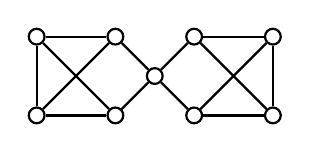
\begin{tikzpicture}[auto,
    specification/.style ={circle, draw, thick, inner sep = 0pt, minimum size=2mm}]
   \node[specification] (A)  at (0,0.5)  {};
   \node[specification] (B)  at (0,-0.5)  {};
   \node[specification] (C)  at (1,0.5)  {};
   \node[specification] (D) at (1,-0.5)  {};
   \node[specification] (E)  at (1.5,0)  {};
   \node[specification] (F)  at (2,0.5)  {};
   \node[specification] (G)  at (2,-0.5)  {};
   \node[specification] (H)  at (3,0.5)  {};
   \node[specification] (I)  at (3,-0.5)  {};
   
   \draw[thick] (A) to  (B);
   \draw[thick] (B) to  (C);
   \draw[thick] (A) to  (D);
   \draw[thick] (A) to  (C);
   \draw[thick] (B) to  (D);

   \draw[thick] (C) to  (E);
   \draw[thick] (D) to  (E);
   
   \draw[thick] (E) to  (F);
   \draw[thick] (E) to  (G);
   \draw[thick] (G) to  (H);
   \draw[thick] (H) to  (I);
   \draw[thick] (I) to  (F);
   \draw[thick] (F) to  (H);
   \draw[thick] (G) to  (I);
 \end{tikzpicture}                     

\end{proof}

  \begin{Exercise}
  有割点的连通图是否一定不是欧拉图?是否一定不是哈密顿图?有桥的连通图是否一定不是欧拉图和哈密顿图?
\end{Exercise}

  \begin{proof}[解]
  有割点的连通图可能为欧拉图;有割点的连通的图一定不是哈密顿图。有桥的连通图一定不是欧拉图;有桥的连通图一定不是哈密顿图。
\end{proof}


\end{CJK}
\end{document}


%%% Local Variables:
%%% mode: latex
%%% TeX-master: t
%%% End:
